% ****** Start of file apssamp.tex ******
%
%   This file is part of the APS files in the REVTeX 4.2 distribution.
%   Version 4.2a of REVTeX, December 2014
%
%   Copyright (c) 2014 The American Physical Society.
%
%   See the REVTeX 4 README file for restrictions and more information.
%
% TeX'ing this file requires that you have AMS-LaTeX 2.0 installed
% as well as the rest of the prerequisites for REVTeX 4.2
%
% See the REVTeX 4 README file
% It also requires running BibTeX. The commands are as follows:
%
%  1)  latex apssamp.tex
%  2)  bibtex apssamp
%  3)  latex apssamp.tex
%  4)  latex apssamp.tex
%
\documentclass[%
 reprint,
superscriptaddress,
%groupedaddress,
%unsortedaddress,
%runinaddress,
%frontmatterverbose, 
%preprint,
%preprintnumbers,
%nofootinbib,
%nobibnotes,
%bibnotes,
 amsmath,amssymb,
 aps,
%pra,
%prb,
%rmp,
%prstab,
%prstper,
%floatfix,
]{revtex4-2}
\usepackage{physics}
\usepackage[dvipsnames]{xcolor}
\usepackage{graphicx}% Include figure files
\usepackage{dcolumn}% Align table columns on decimal point
\usepackage{bm}% bold math
\usepackage{hyperref}% add hypertext capabilities
%\usepackage[mathlines]{lineno}% Enable numbering of text and display math
%\linenumbers\relax % Commence numbering lines
\newcommand{\vvv}[1]{\textcolor{blue}{#1}}
%\usepackage[showframe,%Uncomment any one of the following lines to test 
%%scale=0.7, marginratio={1:1, 2:3}, ignoreall,% default settings
%%text={7in,10in},centering,
%%margin=1.5in,
%%total={6.5in,8.75in}, top=1.2in, left=0.9in, includefoot,
%%height=10in,a5paper,hmargin={3cm,0.8in},
%]{geometry}
\begin{document}

\preprint{APS/123-QED}

\title{Blueprint for efficient nuclear spin characterization in  color center}% Force line breaks with \\
%\thanks{A footnote to the article title}%

\author{Majid Zahedian}
 \affiliation{3rd physical institute University of Stuttgart, Germany}
  %\affiliation{Max Planck School of Photonics, Germany}%Lines b%Lines break automatically or can be forced with \\


\author{Vadim Vorobyov}
\email[]{v.vorobyov@pi3.uni-stuttgart.de}
 \affiliation{3rd physical institute University of Stuttgart, Germany}  
% with \\

 
\author{J\"org Wrachtrup}
 \affiliation{3rd physical institute University of Stuttgart, Germany}%Lines break 
 \affiliation{Max Planck Institute for solid state physics, Stuttgart, Germany}%Lines break 
 %automatically or can be forced with \\ Third institution, the second for Charlie Author

\date{\today}% It is always \today, today,
             %  but any date may be explicitly specified

\begin{abstract}
Nuclear spins in solids is one of the most promising platforms for realisation of a scalable quantum hardware. They could be efficiently adressed at single site level by nearby single colour centers via the spin resonance. However, characterising each nuclear spin is quite cumbersome as the characterisation protocol may differ depending on the strength of the hyperfine coupling. The most adopted protocol is modified electron spin Hahn-echos such as CPMG and XY8 pulse sequences. In some cases, e.g. for spin 1/2, strongly coupled spins, and bispecies bath this protocol contains severe problems in applying for the nuclear spin bath characterisation. 
Here, we present a more straight forward method to obtain hyperfine interaction among nuclear spins and the electron spin. 
This method can be used for a variety of platform including emerging S=1/2 group IV defects in diamond (e.g. SiV, GeV, SnV, PbV) or Silicon vacancy in Silicon Carbide.
We summarize theoretical framework and adopt it from ESR for the use in colour centers with various spins, and numerically consider case of nuclear spin cluster, as compare performance of various protocols on this example via the Fisher information matrix. 
\end{abstract}

%\keywords{Suggested keywords}%Use showkeys class option if keyword
                              %display desired
\maketitle
%\tableofcontents
\section{Introduction and background}
Optically active defects in solids, color centers, has been applied for realising different quantum applications \cite{awschalom2018quantum}, such as a quantum network \cite{pompili2021realization}, quantum sensing \cite{degen2017quantum}, and quantum registers \cite{bradley2019ten}. 
Each center contains an electron spin that can be controlled directly with microwaves, aligned and read via optics. 
The key element for most applications is that they could be coupled through the hyperfine coupling to the bath of numerous nuclear spins presenting a long living quantum memories and could present a nuclear spin qubit register. 
To design the efficient quantum control for the memories, a precise knowledge of the full hamiltonian of the register needs to be known and characterised before. 
However, characterising the nuclear spin hyperfine coupling could be a challenge and a lengthy procedure. 

is necessary for enlarging the quantum register and precise description of the electron spin dynamics. Traditionally, nuclear spin characterisation is done with Optically Detected Magnetic Resonance (ODMR) (ref to Phillip Neumann's works), however the spectroscopic resolution is limited to the $T_2^\ast$ of the electron spin. Hence, some sequence is needed to increase the resolution. People have used Hahn Echo sequence to refocus the electron spin and enhance the coherence time of the electron spin \cite{childress2006coherent}. But this method only works for defects with a specific nuclear spins configuration. Depending on the applied protocol for nuclear spins characterization, the number of accessible nuclear spin can increase. Electron Spin Echo Envelop Modulation (ESEEM) types of sequences allow us to access the highest number of nuclear spins since the spectroscopy resolution is limited to the longitudinal relaxation time ($T_1$) of the system (see fig. \ref{fig:1}). 
\begin{figure*}%[htbp]
	\begin{center}
		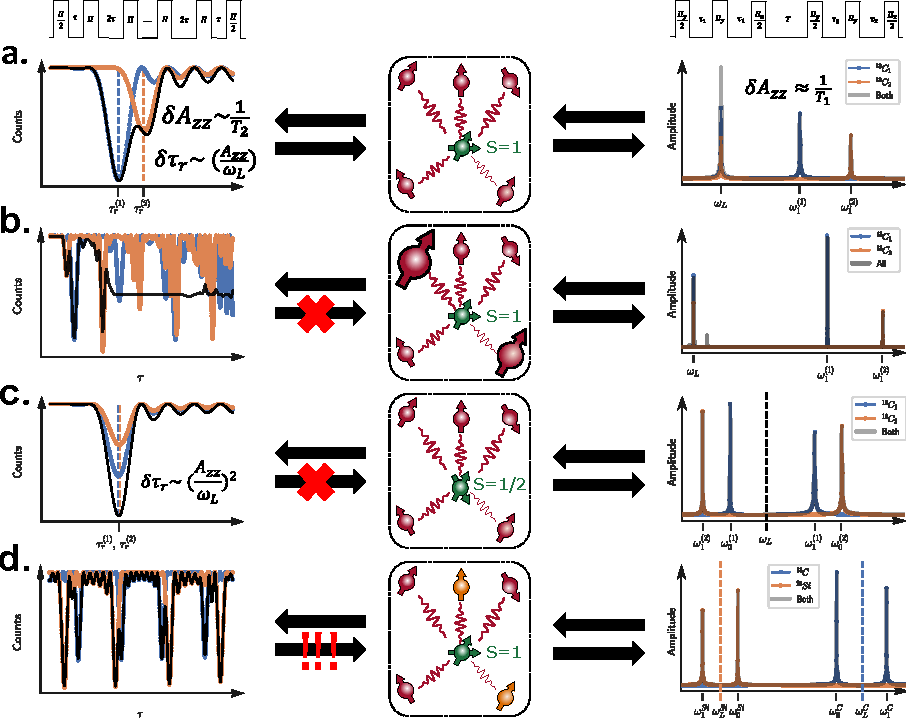
\includegraphics[width=0.9\textwidth]{pict/drawing0.pdf}
		\caption{Comparing DD and 5pESEEM as two nuclear spin characterization method in different systems. a. An electron spin one system: in DD signal, each nuclear spin has a distinct resonance time up to first order of $A_{zz}$; the accuracy of the obtained hyperfine interaction is limited to $T_2$ of the electron spin. In the Fourier transform of the ESEEM signal, the two resonance frequency of each spin is present; the accuracy of the obtained hyperfine interaction is limited to $T_1$ of the electron spin b. An electron spin one system with two strongly coupled nuclear spins and many weakly coupled spins. No resonance time is detectable since the required condition for DD ($\omega_L \gg A_{zz}, A{zx}$) does not hold. However, resonant frequencies is still obtainable in the ESEEM signal c. An electron spin one half system: nuclear spins have more or less the same resonance time as it depends on the second order of hyperfine coupling. However, resonant frequency of each spins is distinguishable in the ESEEM signal. d. A system containing two different nuclear spin species: two nuclear spin bath can interfere in the DD signal, which makes the signal analysis more challenging. However, the species can be inferred from ESEEM signal since species have different Larmor frequencies.}
		\label{fig:1}
	\end{center}
\end{figure*}




%%%%%%%%%%%%%%%%%%%================= %THEORY
\section{Methods}
\label{sec:theory}
%%%%%%%%%%%%%%%Í%%%%=================
In this section, we provide the theoretical formulas for. In a central electron spin with the electron spin $\boldmath{S}$, we only apply pulses resonant with two of the electron spin sublevels, denoted as $m_s=s_0$ and $m_s = s_1$. These two spin sublevels are separated, due to Zeeman effect or zero field splitting, and form an artificial two-level system with energy splitting of $\omega_a$. Now, we add spin $\frac{1}{2}$nuclear spins to the system (for considering P1 centers, one has to add nuclear quadrupole to the presented Hamiltonian.). The Hamiltonian of a central electron spins system surrounded by nuclear spins in the secular approximation in the rotating frame of the applied microwave $\omega_{mw}$ (considering rotating wave approximation) can be written as:
\begin{align}
	H = \Delta S_z + \sum_k (\omega_L^{(k)}  + A_{zz}^{(k)} S_z) I_z^{(k)} + A_{zx}^{(k)} S_z I_x^{(k)}
	\label{eq:H}
\end{align}
Where $\Delta = \omega_a - \omega_{mw}$ is the detuning, $\omega_L^{(k)} =\gamma_n^{(k)} B$ is nuclear Rabi frequency with $\gamma_n^{(k)}$ nuclear spin gyromagnetic ratio and $B$ external magnetic field, $A_{zz}, A_{zx}$ parallel and perpendicular secular component of hyperfine tensor. This Hamiltonian results that depending on the electron spin sublevel $s_i$ ($i=0,1$), the nuclear spin rotate with the resonance frequency of $\omega_i = \sqrt{(\omega_L + s_i A_{zz})^2+ (s_i A_{zx})^2}$, $i=0,1$ along the axes $\vec{n}_i =(\frac{s_i A_{zx}}{\omega_i}, 0, \frac{\omega_L + s_i A_{zz}} {\omega_i})$. It is assumed that the pulse duration $t_p$ are short enough ($\omega_L t_p \ll 1$) that the nuclear spin dynamics during this time is negligible. The most simplest characterization sequence is Ramsey. \\ The Ramsey signal can be obtained as follows:
\begin{gather}
	\expval{\sigma_z}_{Ram} = \cos(\Delta \tau) \prod_{k=1}^{n} \Big[ \cos(\frac{\omega_0 \tau}{2}) \cos(\frac{\omega_1 \tau}{2})+ \notag \\
	(\vec{n_0}\cdot \vec{n_1})\sin(\frac{\omega_0 \tau}{2}) \sin(\frac{\omega_1 \tau}{2}) \Big]^{(k)}
	\textcolor{gray}{e^{-\frac{\tau}{T_2^\ast}}}
\end{gather} 
We do not take any relaxation process into account and the gray exponential decay is put by hand to remember the relaxation time scale. Ramsey signal decay with electron spin $T_2^\ast$, so it can be used to observe the core of the defect. Ramsey sequence is sensitive to detuning since the electron spin is not refocused, however it is possible to sense nuclear spins with vanishing perpendicular hyperfine coupling.\\

To enhance the relaxation time and have access to more nuclei, one can add a $\pi$ pulse in between the Ramsey sequence and create Hahn-echo sequence and obtain the following signal:
\begin{gather}
	\expval{\sigma_z}_{HE} = \prod_{j=1}^n \Big[1 - 2 k^2 
	\sin^2(\frac{\omega_0 \tau}{2}) \sin^2(\frac{\omega_1 \tau}{2})\Big]^{(j)} \textcolor{gray}{ e^{-\frac{2\tau}{T_2}}}
\end{gather}
Where $k = \frac{(s_1-s_0)\omega_L A_{zx}}{\omega_0 \omega_1}$ is the modulation amplitude of each nuclear spin. We know that without any nuclear spin, Hahn Echo sequence creates the electron spin echo signal with the envelope of exponential decay with $T_2^{HE}$. However in the presence of nuclear spins, the electron spin echo envelope will be modulated due to interaction with nuclei. Hence, this sequence also called Electron Spin Echo Envelope Modulation or shortly ESEEM. Even though the coherence time is increased, distinguishing the effect of different nuclear spins in the total signal is very complicated. Hahn Echo sequence can be used for defects that contain a few strongly coupled nuclei. In order to differentiate the resonance frequency of each nuclear spin or make the oscillation sharper, one has to add more $\pi$ pulses and for the so-called Dynamical Decoupling sequence:
Finally, the signal for dynamical decoupling is obtained:
\begin{gather}
	\expval{\sigma_z}_{DD} =
	\prod_{j=1}^n \Big[1- 2 k^2  
	\sin^2(\frac{\omega_0 \tau}{2}) \sin^2(\frac{\omega_1 \tau}{2}) \frac{\sin^2(\frac{N}{2} \theta)}{\cos^2(\frac{1}{2}\theta)}  \Big]^{(j)} \textcolor{gray}{ e^{-\frac{2N\tau}{T_2(N)}}} 
\end{gather}
Where
\begin{gather}
	\theta=  \arccos\Big[\cos(\omega_0 \tau) \cos(\omega_1 \tau)- \vec{n}_0 \cdot \vec{n}_1 sin(\omega_0 \tau) \sin(\omega_1 \tau) \Big]
\end{gather}
$\vec{n}_0 \cdot \vec{n}_1 = \frac{\omega_L^2+(s_0+s_1)A_{zz}+s_0 s_1 (A_{zz}^2+A_{zx}^2)}{\omega_0 \omega_1}$ and $N$ is the number of $\pi$ pulses that must be an even. Each nuclear 
If the magnetic field is high or all nuclear spins are weakly coupled such that $\omega_L \gg A_{zz}, A_{zx}$, the multiplication rule can be approximated by a summation rule, which makes the higher order resonance disappear:
\begin{gather}
	\expval{\sigma_z}_{DD} \approx 1 -2
	\sum_{j=1}^n \Big[ k^2 	 \sin^2(\frac{\omega_0 \tau}{2}) \sin^2(\frac{\omega_1 \tau}{2}) \frac{\sin^2(\frac{N}{2} \theta)}{\cos^2(\frac{1}{2}\theta)}  \Big]^{(j)} \textcolor{gray}{ e^{-\frac{2N\tau}{T_2(N)}}} 
\end{gather}
The parallel component of the hyperfine interaction can be obtained from the resonance time of each nuclear spin:
\begin{gather}
	\tau_p \approx  \frac{(2p+1) \pi}{\omega_0 + \omega_1} \approx \frac{(2p+1)\pi}{2\omega_L(1+\frac{s_0+s_1}{2} \frac{A_{zz}}{\omega_L}+ \frac{s_0^2+s_1^2}{4}\frac{A_{zx}^2}{\omega_L^2})}
\end{gather}
The perpendicular part of hyperfine interaction can be obtained from a fit to the Lorentzian dip with the width of $\frac{(s_1-s_0)\omega_L A_{zx}}{(2p+1)\pi\omega_0 \omega_1}$ or varying the number of pulses and fitting the minima position to the formula $\expval{\sigma_z}_{DD}^{(k)} \approx 1- 2 \sin^2\big(\frac{N}{2}\frac{(s_1-s_0)\omega_L A_{zx}}{\omega_0 \omega_1}\big) $. Although Dynamical Decoupling (DD) sequence is well understood and used to characterize nuclear spins, it is not applicable for any system. First, DD only works for defects with high magnetic field and low hyperfine coupling ($\omega_L \gg A_{zz}, A_{zx}$). Second, the signal is limited to electron spin $T_2$, which is difficult to make it equal to $T_1$. Third, the signal analysis is rather complicated and time-consuming. (Maybe AI solves this problem in the future?) one has to collect enough data to make sure no two nuclear spin overlap in the signal. Forth, this sequence does not work for spin one half system, e.g., group IV defect in diamond, since parallel component of hyperfine coupling cancels their effect in the resonance time up to the first and second order. Hence, the resonance time depends on the second order of perpendicular component. In this work, we take 23 nuclear spin characterized in paper \cite{abobeih2019atomic} as a realistic case. 
\begin{figure}%[htbp]
	\begin{center}
		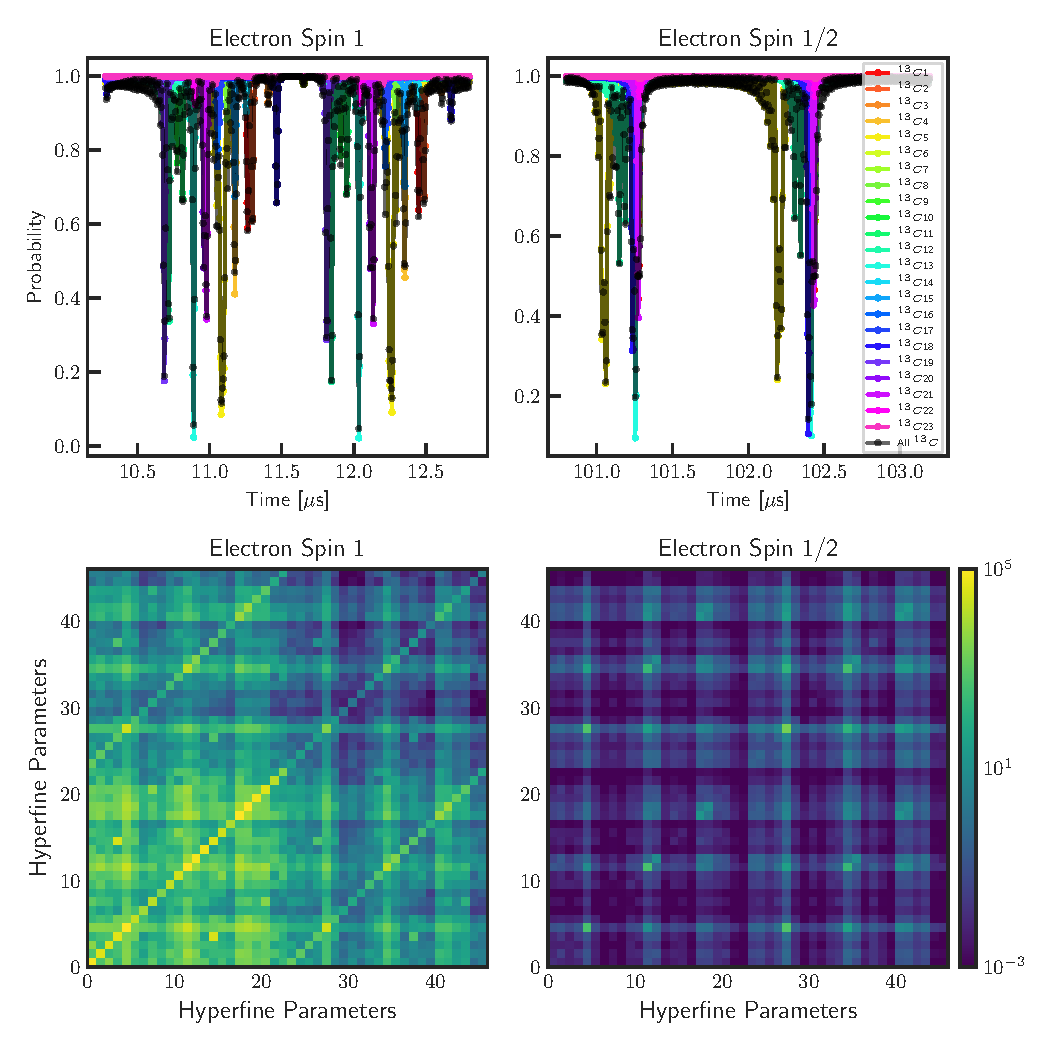
\includegraphics[width=0.9\columnwidth]{pict/dd_compare2.pdf}
		\caption{Simulated DD signal with 64 $\pi$-pulses for the register reported \cite{abobeih2019atomic} assuming the electron spin is a. spin one b. spin one-half system. Simulated Fisher information for the case of the electron spin c. one d. one-half system.}
		\label{fig:3}
	\end{center}
\end{figure}
Fig \ref{fig:3} compares DD signal for the same nuclear spin register but different defects in diamond. We present a handwavy definition for the sensitivity of a sequence to the variation of hyperfine coupling. First, we consider the case of NV center in diamond. By knowing the width of a dip $\delta \tau = \frac{A_{zx}}{\omega_L^2}$  and taking the derivative of the resonance time, we define the sensitivity of longitudinal hyperfine coupling as follows:
\begin{gather}
	\delta A_{zz} = \frac{\delta \tau}{\abs{\frac{\partial \tau_k}{\partial A_{zz}}}} = \frac{2}{\tau_k} \frac{A_{zx}}{\omega_L} \ge \frac{4}{T_2^{HE}} \frac{A_{zx}}{\omega_L}
\end{gather}
If we assume the typical values of $T_2^{HE} = 100 $ $\mu$s and $\omega_L=500 $ kHz, a weakly coupled nuclear spin $A_{zx}=5$ kHz can be distinguished from another weakly coupled nuclear spin with $\delta A_{zz} = 400$ Hz. On the other hand, for group IV detects in diamond, The resonance times is sensitive to the second order of $A_{zx}$ and no sensitivity to $A_{zz}$. Hence, even at large $\tau$ the nuclear spin not separated well. We define the sensitivity for the spin one half system as follows:
\begin{gather}
	\delta A_{zx} = \frac{\delta \tau}{\abs{\frac{\partial \tau_k}{\partial A_{zx}}}} = \frac{4}{\tau_k} \ge \frac{8}{T_2^{HE}}
\end{gather}
Assuming the typical values of $T_2^{HE} = 100 $ $\mu$s, a nuclear spin can be distinguished from another one if their transverse hyperfine coupling is separated by $\delta A_{zx} = 80$ kHz, which is quite inaccurate.\\

   
We want to make a sequence that is limited by T1 instead of T2. The idea of 5-pulse ESEEM \cite{kasumaj20085} is that to create an entanglement (Hahn-echo) before the free evolution (Ramsey). In other words, change the initial density matrix for the Ramsey sequence from such that entanglement already exist in the electron polarization terms of the density matrix. Fig \ref{fig:seqs} shows the sequence, which can be interpreted as two Hahn Echos that are separated by a long free evolution $T\gg T_2^\ast$ such that the coherence of the electron spin vanishes. The analytical formula to this sequence is provided in the appendix \ref{app:5pESEEM}. During the free evolution time, each nuclear spins oscillates with either of two resonance frequencies obtained from eq. \ref{eq:H}.

\begin{figure*}[htbp]
	\begin{center}
		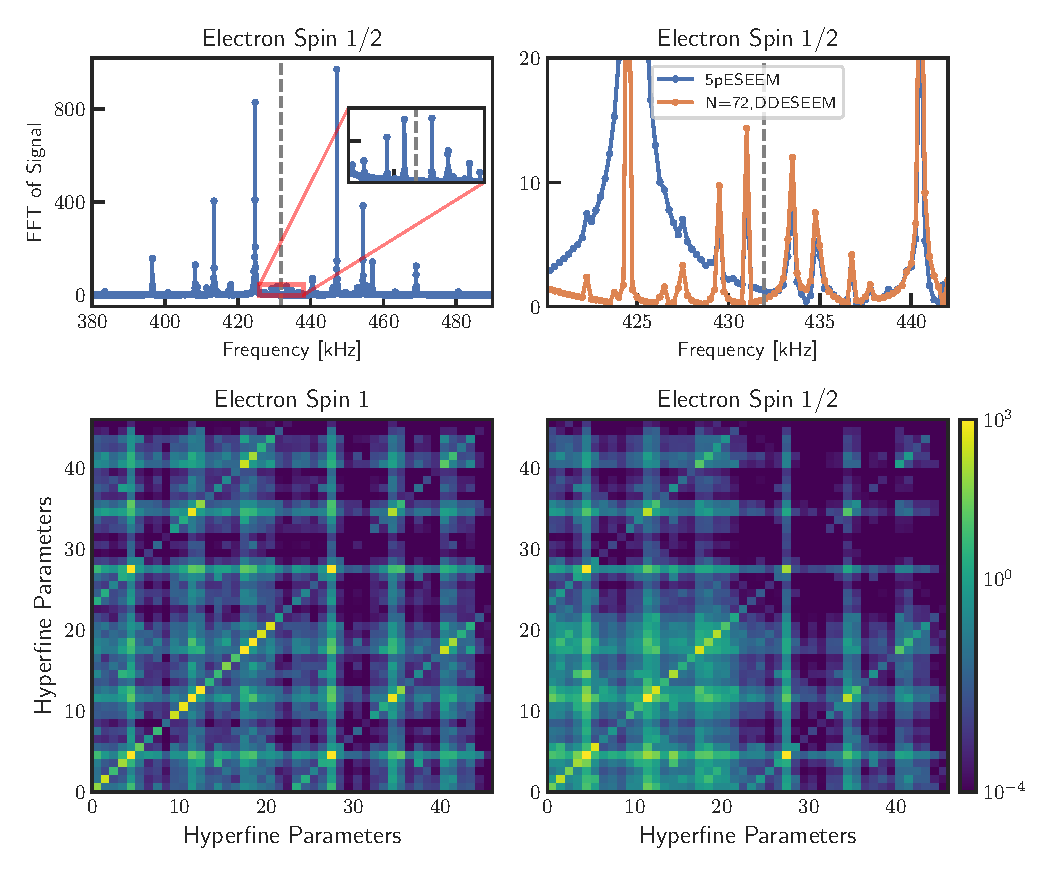
\includegraphics[width=0.9\textwidth]{pict/eseem_compare2.pdf}
		\caption{Simulated FFT of ESEEM signal with a zoom into weakly coupled nuclear spins for the register reported \cite{abobeih2019atomic} assuming the electron spin is one-half. b. Enhancing the sensitivity to weakly coupled spins by increasing number of $\pi$-pulses to $N=72$ pulses in each entangling period. $\tau$ is set to the Larmor bright spot. Simulated Fisher information for the case of the electron spin c. one d. one-half system.}
		\label{fig:4}
	\end{center}
\end{figure*}

>>>>>>> c0eaca02ca59681a3dedd48a17843824ce2f8aac
Fig \ref{fig:4} shows the furrier transform of the signal. Zooming into area close to the Larmor frequency reveals the weakly coupled nuclei. Each nuclear spins have two peaks in the spectrum. Expanding the resonance frequencies up to first order with respect to hyperfine coupling results that the weakly coupled nuclei keep their order as they go further away from the nuclei. This fact makes their characterization rather straight forward. To observe the weakly coupled nuclei more pronouncedly, one can use DDESEEM sequence by adding more $\pi$ pulses in the entangling periods. To distinguish other nuclei, extra measurements is required. One method is to use two dimensional hyperfine correlation spectroscopy (2D Hyscore)  \cite{vorobyov2022addressing}. However, this method is rather time-consuming as two time variables has to be swept. We suggest sweeping $\tau$ parameter and keep the track of frequency amplitude as a function of $\tau$. Two frequencies that belong to the same nuclear are correlated because the modulation depth oscillates with blind spot terms of both frequencies $\sin^2(\frac{\omega_0 \tau}{2}) \sin^2(\frac{\omega_1 \tau}{2})$. Fig. \ref{fig:5} shows two frequencies goes to bright and blind spots simultaneously. Hence, taking two dimensional correlation of the spectrum, one can deduce which two frequencies are correlated and belong to the same nuclear. \\

Here, we try to simulate the realistic situation. First, the electron spin state is projected to 0 and 1 with a binomial distribution, the probability determined by the theoretical signal. Then, we assume the bright (dark) state emits 3 (0.1) photons on average with a Poissonian distribution. We repeat the measurement at each point for 10000 times to reduce classical noise.\\
How many nuclear spin is identifiable with this method? It depends on the duration of free evolution time and the choice of inter-pulse timing $\tau$.

\begin{figure*}%[htbp]
	\begin{center}
		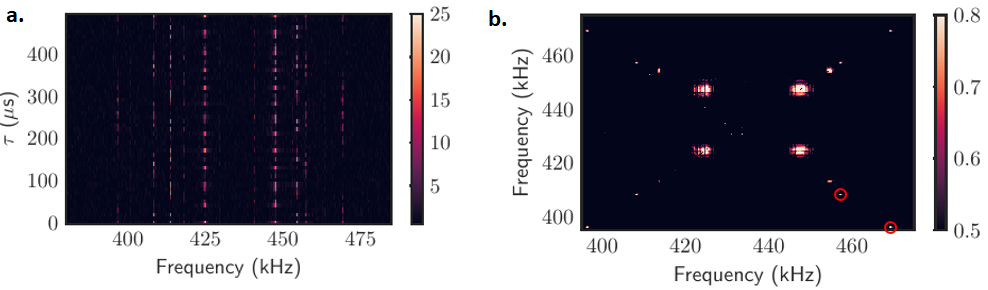
\includegraphics[width=0.9\textwidth]{pict/fig5.png}
		\caption{a. FFT of ESEEM signal for $\tau$ from 10 $\mu$s to 500 $\mu$s with the step of 10 $\mu$s b. 2D correlation of each frequency for different $\tau$.}
		\label{fig:5}
	\end{center}
\end{figure*}

\section{Conclusion}
\label{sec:discussion}
%\subsection{Advanced filters}
Here is the concise conclusion @Vadim


\section*{Acknowledgments}
We acknowledge financial support by European Union's Horizon 2020 research and innovation program ASTERIQS under grant No. 820394, European Research Council advanced grant No. 742610, SMel, Federal Ministry of Education and Research (BMBF) project MiLiQuant and Quamapolis, the DFG (FOR 2724), the Max Planck Society, and the Volkswagentiftung. M.Z. thanks Max Planck School of Photonics for financial support.


%%%%%%%%%%%%%=========
\appendix
%%%%%%%%%%%%%=========
\section{5pESEEM formula}
\label{app:seqs}
The details of mentioned sequences in the main text can be found in fig \ref{fig:seqs}:
\begin{figure}%[htbp]
	\begin{center}
		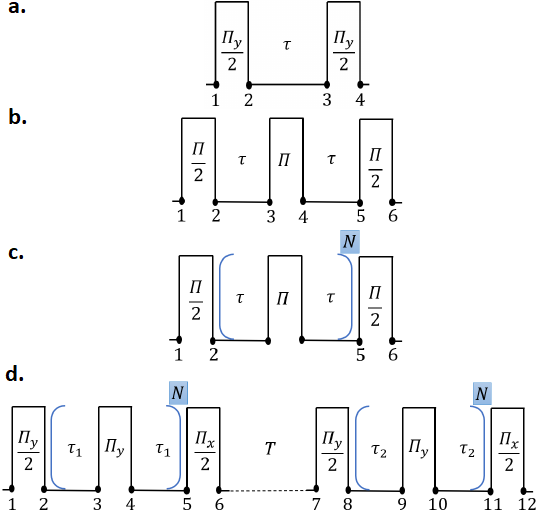
\includegraphics[width=0.9\columnwidth]{pict/seqs.png}
		\caption{Pulse sequences a. Ramsey b. Hahn Echo c. Dynamical Decoupling d. DDESEEM}
		\label{fig:seqs}
	\end{center}
\end{figure}

\section{5pESEEM formula}
\label{app:5pESEEM} 
Here we need to define a few unitary operators/ The evolution in the first Hahn-echo is given by V operators, the middle free evolution is given by F operators, and the second Hahn-echo is given by W operators:
\begin{gather}
	V_0 = U_0 (\tau_1) U_1 (\tau_1),\,\,  V_1 = U_1 (\tau_1) U_0 (\tau_1) \\
	F_0 = U_0 (T), \,\, F_1 = U_1 (T) U_0 \\
	W_0 = U_0 (\tau_2) U_1 (\tau_2), \,\, W_1 = U_1 (\tau_2) U_0 (\tau_2)
\end{gather}
The signal can be obtained from four different types of trajectories that the electron spin can take. We use the fact that multiplication of unitary operators is also a unitary operator and every unitary in spin one half space can be written in terms of a rotation angle, axis, and Pauli Matrices $\vec{\sigma}$. We denote the unitary operator $U = \exp(-i \theta_U \hat{n}_U\cdot\vec{\sigma}) = M\cos(\theta_U) \mathbf{I}- i \sin(\theta_U) \hat{n}_U\cdot\vec{\sigma}$. The signal for 5-pulse ESEEM can be obtained as follows:
\begin{gather}
		\expval{\sigma_z}_{5p} =\frac{1}{4}\Big( \prod_{j=1}^n [\cos(\theta_{W_1 F_1 V_0 V_1^\dagger F_1^\dagger W_0^\dagger})]^{(j)}  \notag \\
		-\prod_{j=1}^n [\cos(\theta_{W_1 F_1 V_1 V_0^\dagger F_1^\dagger W_0^\dagger})]^{(j)}  \notag \\
		+ \prod_{j=1}^n [\cos(\theta_{W_1 F_0 V_0 V_1^\dagger F_0^\dagger W_0^\dagger})]^{(j)}  \notag \\
		-\prod_{j=1}^n [\cos(\theta_{W_1 F_0 V_1 V_0^\dagger F_0^\dagger W_0^\dagger})]^{(j)} \Big) \textcolor{gray}{e^{-\frac{2\tau_1+2\tau_2}{T_2}- \frac{T}{T_1}}}
\end{gather}
Multiplying the matrices and finding the rotation angles gives the expectation value of $\sigma_z$ for 5pESEEM sequence as it can be found in this article \cite{kasumaj20085}:
\begin{gather}
	\expval{\sigma_z}_{5p} = \frac{1}{4}\Big( \prod_{j=1}^n E_{\alpha_+}^{(j)} - \prod_{j=1}^n E_{\alpha_-}^{(j)} + \prod_{j=1}^n E_{\beta_+}^{(j)}- \prod_{j=1}^n E_{\beta_-}^{(j)}\Big)
\end{gather}
Where each term can be calculated as follows:
\small   
\begin{gather} 
	E_{\alpha_\pm}^{(k)} = E_{2p}(\tau_1) E_{2p}(\tau_2) \mp B \Big(-4k^2C_\alpha \notag \\
	+4k\cos^4(\eta) \cos(\omega_\alpha T + \phi_{\alpha_+} +\phi_{\beta_+}) 
	+2 k^2 \cos(\phi_{\beta_-}) \cos(\omega_\alpha T+\phi_{\alpha_+}) \notag \\
	+ 4k \sin^4(\eta) \cos(\omega_\alpha T +\phi_{\alpha_+} -\phi_{\beta_+} )\Big)
	\label{eq:eseem}
\end{gather}
\normalsize
$ E_{2p} $ is 2-pulse ESEEM sequence signal:
\begin{gather}
	E_{2p}(t)  = (1 - \frac{k}{2}) + \frac{k}{2} \Big(\cos(\omega_\alpha t)+\cos(\omega_\beta t) \notag \\
	-\frac{1}{2} \cos(\omega_{-}t)  -\frac{1}{2} \cos(\omega_{+}t)   \Big)
\end{gather}
With $\omega_{\pm} = \omega_\alpha \pm \omega_\beta$,  B is the blind spot term and $C_\alpha$ is a constant term:
\begin{gather}
	B = \sin(\frac{\omega_\alpha \tau_1}{2}) \sin(\frac{\omega_\alpha \tau_2}{2}) \sin(\frac{\omega_\beta \tau_1}{2}) \sin(\frac{\omega_\beta \tau_2}{2})
	\label{eq:BS}\\
	C_\alpha =\cos(\frac{\omega_\alpha \tau_1}{2}) \cos(\frac{\omega_\alpha \tau_2}{2}) \sin(\frac{\omega_\beta \tau_1}{2}) \sin(\frac{\omega_\beta \tau_2}{2}) \label{eq:Cterms}
\end{gather}
The resonance frequencies are $\omega_{\alpha(\beta)} = \sqrt{(\omega_L +s_{0(1)} A_{zz} )^2 +(s_{0(1)} A_{zx})^2}$. The quantization axis of nuclear spins is tilted by $\eta_{\alpha(\beta)} = \arctan(\frac{s_{0(1)}A_{zx}}{\omega_L+ s_{0(1)}A_{zz}})$, which gives the parameter $\eta=\frac{\eta_\alpha - \eta_\beta}{2}$. The modulation depth of each nuclear spin is $k=\sin^2(2\eta)=(\frac{(s_1-s_0)\omega_L A_{zx}}{\omega_\alpha \omega_\beta})^2$, the phase shifts are $\phi_{\alpha_\pm} = \frac{\omega_\alpha (\tau_1 \pm \tau_2)}{2}$ and $\phi_{\beta_\pm} = \frac{\omega_\beta (\tau_1 \pm \tau_2)}{2}$. The two expression for the $\beta$ pathways can be obtained by exchanging $\alpha$ and $\beta$ in equation \ref{eq:eseem}, \ref{eq:BS}, and \ref{eq:Cterms}.\\


As we have shown, the signal from the register comes from the multiplication of signals from individual nuclear spins. Hence, if the modulation depth is not low (low magnetic field condition), the second or higher order frequencies will appear in the spectrum. So, the product rule lead to the creation of inter-nuclear peaks at multi-quantum frequencies that can be sums or subtraction of single quantum frequencies of various nuclei. Nevertheless, the multiple quantum resonance peaks are informative for the electron spin one half system because one can deduce that two peaks that are added or subtracted belong to the same electron spin manifold; Hence it is possible to get the relative phase of nuclei. Another consequence of the product rule is the cross-suppression effect, which means the presence of strongly coupled nuclei suppress the amplitude of weakly coupled nuclei while weakly coupled ones do not suppress the amplitude of strongly coupled nuclei \cite{stoll2005peak}. However, if we assume the Larmor frequency is relatively high or the modulation depth is low, both of these effect will vanish as the product rule can be approximated by a summation rule:\\
\begin{gather}
	E_\alpha = \prod_{j=1}^n E_{\alpha_+}^{(j)} - \prod_{j=1}^n E_{\alpha_-}^{(j)}  \notag \\ 
	\approx \sum_{j=1}^n \Big[-8Bk\cos^4(\eta) \cos(\omega_\alpha T + \phi_{\alpha_+}+ \phi_{\beta_+}) \Big]^{(j)}
\end{gather}

The blind spot term shows that how this sequence can be engineered to increase or reduce the signal amplitude of one nuclear spin from the spectrum. The bright and blind spots of a frequency in the spectrum are as follows:
\begin{align}
	\text{Blind Spots:	} \tau = even \,\, \frac{\pi}{\omega}\\
	\text{Bright Spots:	} \tau = odd \,\, \frac{\pi}{\omega}
\end{align}
The blind spots does not depend only on one frequency but on the nuclear spin. It means if one resonant frequency is blinded, the other resonant frequency and all the multiple quantum resonances also vanishes. This can be used as a manifestation that which two peaks are from one nuclei. Also, This is very helpful especially in the presence of strongly coupled nuclear spin that suppress other nuclei. By sweeping $\tau_1$ and $\tau_2$, one can go through different bright and blind spots of each nuclear spin, observe which two peaks are correlated.

%pass
\bibliography{references}% Produces the bibliography via BibTeX.


% The \nocite command causes all entries in a bibliography to be printed out
% whether or not they are actually referenced in the text. This is appropriate
% for the sample file to show the different styles of references, but authors
% most likely will not want to use it.
%\nocite{*}
\end{document}
%
% ****** End of file apssamp.tex ******